\section{历史条件下的随机累计}
\label{sec:dtsp-accumulation}

前两节研究完整的条件分布：给定现在，未来怎样分布。很多问题只需要更少的信息。赌徒关心每局的期望输赢，算法关心每步更新平均朝哪里走，误差分析关心累计波动有多大。本节把注意力从条件分布转向条件均值，把每一步增量拆成两部分：一部分在增量出现之前就可以由历史预测，称为漂移；另一部分给定历史后平均为零，是无法用过去消除的噪声。只含后者的累计量就是鞅，它是后面停止、偏差控制与收敛分析的共同对象。

\subsection{鞅、次鞅与超鞅}
\label{sec:dtsp-martingales}

\paragraph{公平游戏的数学表达}
设$\xi_1,\xi_2,\ldots$独立，各以$1/2$的概率取$\pm1$，令$S_0=0$、$S_n=\sum_{k=1}^n\xi_k$，滤过取$\mathcal F_n=\sigma(\xi_1,\ldots,\xi_n)$。把$S_n$看成反复押一元硬币的累计输赢。无论之前赢了多少，下一局的条件期望输赢都是零：
\[
  \mathbb E[S_{n+1}\mid\mathcal F_n]=S_n+\mathbb E[\xi_{n+1}\mid\mathcal F_n]=S_n+\mathbb E\xi_{n+1}=S_n.
\]
第二个等号用了$\xi_{n+1}$与$\mathcal F_n$独立。“已知到现在为止的一切，对下一时刻的最佳平均预测就是现在的值”，这就是公平游戏的数学表达。

\begin{definition}[鞅、次鞅与超鞅]
  \label{def:dtsp-martingale}
  设实值过程$(M_n)_{n\geq0}$适应于滤过$(\mathcal F_n)$，且每个$M_n$可积。若对所有$n\geq0$，
  \begin{equation}
    \mathbb E[M_{n+1}\mid\mathcal F_n]=M_n\qquad\text{几乎必然},
    \label{eq:dtsp-martingale}
  \end{equation}
  则称$(M_n)$为相对于$(\mathcal F_n)$的\term{鞅}（martingale）。若等号换成“$\geq$”，称为\term{次鞅}（submartingale）；换成“$\leq$”，称为\term{超鞅}（supermartingale）。鞅的增量$D_n=M_n-M_{n-1}$满足$\mathbb E[D_n\mid\mathcal F_{n-1}]=0$，称为\term{鞅差}（martingale difference）。
\end{definition}

可积性保证条件期望有定义，适应性保证$M_n$在时刻$n$已经可知。反复使用塔式性质，式~\eqref{eq:dtsp-martingale}推出$\mathbb E[M_{n+k}\mid\mathcal F_n]=M_n$对所有$k\geq0$成立，特别地$\mathbb EM_n=\mathbb EM_0$：鞅的期望不随时间改变。次鞅的期望单调不减，超鞅的期望单调不增。名称容易记反：超鞅“平均向下”，像对赌徒不利的赌场；次鞅“平均向上”。

\paragraph{几个基本例子}
下面的例子在后文会反复出现，每个都对应一种构造鞅的方式。
\begin{enumerate}
  \item 中心化累计和。若$\xi_k$独立可积、均值为$\mu$，则$S_n-n\mu$是鞅。向右概率为$p$的$\pm1$游走中$\mu=2p-1$；$p<1/2$时$S_n$本身是超鞅。
  \item 乘积。若$Y_k\geq0$独立且$\mathbb EY_k=1$，则$M_n=\prod_{k=1}^nY_k$是鞅，因为$\mathbb E[M_{n+1}\mid\mathcal F_n]=M_n\mathbb EY_{n+1}$。取$Y_k$等概率为$0$或$2$，得到“加倍或清零”的赌局，它将在第~\ref{sec:dtsp-martingale-limits}节说明鞅的极限与期望可以分离。
  \item 信息逐步揭示。若$Z$可积，则$M_n=\mathbb E[Z\mid\mathcal F_n]$是鞅，由塔式性质直接验证。它表示随信息增加不断修正的最佳预测，称为Doob鞅。
  \item 凸函数。若$(M_n)$是鞅、$\varphi$凸且$\varphi(M_n)$可积，条件Jensen不等式给出$\mathbb E[\varphi(M_{n+1})\mid\mathcal F_n]\geq\varphi(M_n)$，所以$\varphi(M_n)$是次鞅。例如$S_n^2$与$|S_n|$都是次鞅。
\end{enumerate}

\paragraph{信息流决定鞅性质}
鞅的定义中出现了$\mathcal F_n$，结论因此依赖声明的信息流。对上面的公平游走，若改用提前一步揭晓的滤过$\mathcal G_n=\sigma(\xi_1,\ldots,\xi_{n+1})$，$S_n$仍然适应，但$\mathbb E[S_{n+1}\mid\mathcal G_n]=S_{n+1}$，通常不等于$S_n$。偷看下一枚硬币的人眼中，这场游戏不再公平。反过来，若一个过程相对于较细的滤过是鞅，那么相对于它自己生成的较粗滤过仍是鞅：对较粗的信息再取一次条件期望即可。

\paragraph{Markov性质与鞅性质的比较}
Markov性质与鞅性质约束不同的对象。前者说给定现在后，未来的整个条件分布不再依赖过去；后者只说下一步的条件均值等于现在。公平游走二者兼有。有漂移的游走与递推~\eqref{eq:dtsp-random-recursion}是Markov链但不是鞅，因为它们的条件均值偏离当前值。反过来，鞅也不必是Markov链：令下注额$H_k=1+|S_{k-1}|$，累计财富$W_n=\sum_{k=1}^nH_k\xi_k$。给定$\mathcal F_n$，下一步是$W_n\pm(1+|S_n|)$，均值为$W_n$，所以$(W_n)$是鞅；但这一条件分布依赖$S_n$，而$S_n$一般不能由$W_n$确定，因此$(W_n)$相对于$(\mathcal F_n)$不是Markov链。鞅性质只管平均，允许波动的大小依赖整段历史。

\subsection{可预测加权与漂移分解}
\label{sec:dtsp-predictable}

\paragraph{鞅变换：事前下注}
赌徒可以根据已有结果改变每局下注额。关键的限制是：第$k$局的下注额必须在这一局开出之前决定。把这一要求写成可测性：若对每个$k\geq1$，$H_k$对$\mathcal F_{k-1}$可测，就称$(H_k)$是\term{可预测过程}（predictable process）。“可预测”不是说$H_k$没有随机性，而是说它可以由第$k$份新噪声到来之前的信息确定。按此下注的累计收益
\begin{equation}
  (H\cdot M)_n=\sum_{k=1}^nH_k(M_k-M_{k-1})
  \label{eq:dtsp-martingale-transform}
\end{equation}
称为\term{鞅变换}（martingale transform）。它是“随机和”的离散版本：权重在增量揭晓之前确定。

\begin{theorem}[鞅变换]
  \label{thm:dtsp-martingale-transform}
  设$(M_n)$是鞅，$(H_k)$可预测，并且每个$H_k(M_k-M_{k-1})$可积（例如每个$H_k$有界）。则$((H\cdot M)_n)_{n\geq0}$是鞅，其中$(H\cdot M)_0=0$。若$(M_n)$是超鞅，$H_k$非负且有界，则$(H\cdot M)$是超鞅。
\end{theorem}

\begin{proof}
$(H\cdot M)_n$适应且可积。由于$H_{n+1}$对$\mathcal F_n$可测，条件期望可以把它当作已知因子提出：
\[
  \mathbb E[(H\cdot M)_{n+1}-(H\cdot M)_n\mid\mathcal F_n]
  =H_{n+1}\,\mathbb E[M_{n+1}-M_n\mid\mathcal F_n].
\]
鞅情形右侧为零。超鞅情形条件期望非正，再乘以非负的$H_{n+1}$仍非正。
\end{proof}

这个定理说的是：在公平游戏中，不存在只依赖过去的下注系统能把期望收益变为正数。图~\ref{fig:dtsp-martingale-transform}比较两种规则。“按符号跟随”在领先时押正、落后时押负，它只用过去，所以$4000$条路径的平均财富始终贴着零，第$200$局时样本平均为$-0.03$，标准误$0.23$。“事后挑选”每局押中刚揭晓的结果，$H_k=\xi_k$，财富一路涨到$n$；它违反了可预测性，证明中“把$H_{n+1}$提出条件期望”那一步失去依据。定理中的可积性同样不可省略；第~\ref{sec:dtsp-optional-sampling}节的加倍下注会说明，缺少适当的可积或有界条件时，“随机长度”的公平游戏可以产生看似必胜的结果。

\begin{figure}[htbp]
  \centering
  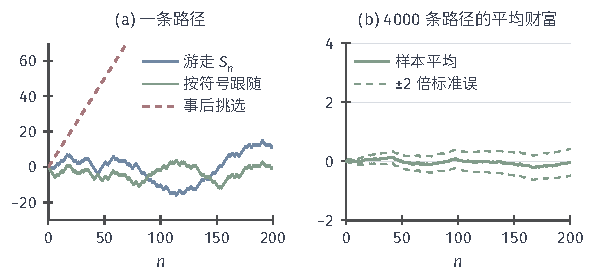
\includegraphics[width=101mm]{figures/03-optimization-evolution-and-signals/02-processes-and-trajectory-evolution/tikz/dtsp-martingale-transform/figure.pdf}
  \caption{事前下注与事后挑选。$S_n$为公平$\pm1$游走。“按符号跟随”取$H_k=\operatorname{sign}(S_{k-1})$（约定$\operatorname{sign}0=1$），只用过去；“事后挑选”取$H_k=\xi_k$，财富等于$n$。(a)一条路径；(b)$4000$条模拟路径上“按符号跟随”的平均财富及其两倍标准误带，始终覆盖零。}
  \label{fig:dtsp-martingale-transform}
\end{figure}

\paragraph{Doob分解：漂移与噪声}
一般的适应过程未必公平。它的每一步增量都可以拆成“事先可预测的平均”与“剩余的意外”。设$(X_n)$适应且可积，令
\begin{equation}
  A_n=\sum_{k=1}^{n}\mathbb E[X_k-X_{k-1}\mid\mathcal F_{k-1}],\qquad
  M_n=X_n-X_0-A_n,
  \label{eq:dtsp-doob-decomposition}
\end{equation}
并约定$A_0=M_0=0$。

\begin{theorem}[Doob分解]
  \label{thm:dtsp-doob-decomposition}
  适应可积过程$(X_n)$可以写成$X_n=X_0+M_n+A_n$，其中$(M_n)$是鞅，$(A_n)$可预测，且$M_0=A_0=0$。这种分解在几乎必然意义下唯一。$(X_n)$是次鞅当且仅当$(A_n)$单调不减；是超鞅当且仅当$(A_n)$单调不增。
\end{theorem}

\begin{proof}
按式~\eqref{eq:dtsp-doob-decomposition}构造，$A_n$的每一项对$\mathcal F_{k-1}\subseteq\mathcal F_{n-1}$可测，所以$A_n$可预测；又
\[
  \mathbb E[M_k-M_{k-1}\mid\mathcal F_{k-1}]=\mathbb E[X_k-X_{k-1}\mid\mathcal F_{k-1}]-(A_k-A_{k-1})=0,
\]
所以$M$是鞅。若另有分解$X_n=X_0+M_n'+A_n'$，则$M_n-M_n'=A_n'-A_n$既是鞅又可预测，于是$M_n-M_n'=\mathbb E[M_n-M_n'\mid\mathcal F_{n-1}]=M_{n-1}-M_{n-1}'$，归纳得它恒等于初值$0$。最后一句由$A_k-A_{k-1}=\mathbb E[X_k-X_{k-1}\mid\mathcal F_{k-1}]$的符号直接读出。
\end{proof}

以公平游走的平方为例。$\mathbb E[S_k^2-S_{k-1}^2\mid\mathcal F_{k-1}]=\mathbb E[2S_{k-1}\xi_k+\xi_k^2\mid\mathcal F_{k-1}]=1$，所以$A_n=n$、$M_n=S_n^2-n$。图~\ref{fig:dtsp-doob-decomposition}把一条路径的$S_n^2$拆成一条直线和一条围绕零波动的曲线；许多路径平均后，$S_n^2$的平均正好贴着漂移线$n$。Doob分解给出后文的标准分析路线：漂移部分用确定性的稳定性或单调性处理，鞅部分用本章后几节的累计偏差与收敛工具处理。第~\ref{sec:dtsp-stochastic-approximation}节的随机递推正是按这条路线分析的。

\begin{figure}[htbp]
  \centering
  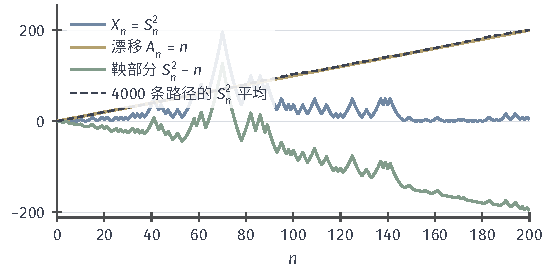
\includegraphics[width=94mm]{figures/03-optimization-evolution-and-signals/02-processes-and-trajectory-evolution/tikz/dtsp-doob-decomposition/figure.pdf}
  \caption{次鞅$S_n^2$的Doob分解。$S_n$为公平$\pm1$游走的一条模拟路径，$S_n^2=(S_n^2-n)+n$分为鞅部分（绿）与可预测漂移$A_n=n$（黄）。黑色虚线是$4000$条模拟路径上$S_n^2$的平均，与$n$几乎重合。}
  \label{fig:dtsp-doob-decomposition}
\end{figure}

\subsection{条件方差与累计波动}
\label{sec:dtsp-quadratic-variation}

\paragraph{鞅增量的正交性}
鞅的均值不变，波动却会累计。设$(M_n)$平方可积，即每个$\mathbb EM_n^2<\infty$。对$j<k$，$D_j$对$\mathcal F_{k-1}$可测，于是
\[
  \mathbb E[D_jD_k]=\mathbb E\bigl[D_j\,\mathbb E[D_k\mid\mathcal F_{k-1}]\bigr]=0.
\]
不同时刻的鞅差在$L^2$中两两正交。把$M_n=M_0+\sum_{k\leq n}D_k$平方后取期望，交叉项全部消失：
\begin{equation}
  \mathbb EM_n^2=\mathbb EM_0^2+\sum_{k=1}^n\mathbb ED_k^2.
  \label{eq:dtsp-orthogonal-increments}
\end{equation}
这是一个“勾股定理”：总长度的平方等于各段正交分量长度平方之和。对公平游走，$\mathbb ES_n^2=n$。

正交不等于独立。在“按符号跟随”或$H_k=1+|S_{k-1}|$这类下注规则中，第$k$步的幅度取决于此前的路径，增量之间显然不独立；但只要条件均值为零，式~\eqref{eq:dtsp-orthogonal-increments}照样成立。把鞅差一律当成独立同分布，会漏掉条件方差随历史变化这一最常见的情形。

\paragraph{可预测二次变差与实现二次变差}
式~\eqref{eq:dtsp-orthogonal-increments}只给出无条件的二阶矩。要描述波动怎样沿路径累计，需要逐步的条件版本。对平方可积鞅，定义
\begin{equation}
  \langle M\rangle_n=\sum_{k=1}^n\mathbb E[D_k^2\mid\mathcal F_{k-1}],\qquad
  [M]_n=\sum_{k=1}^nD_k^2.
  \label{eq:dtsp-quadratic-variations}
\end{equation}
$\langle M\rangle_n$称为\term{可预测二次变差}（predictable quadratic variation），它的每一项在第$k$步发生之前就已知，像一份预先登记的“波动预算”；$[M]_n$称为\term{实现二次变差}（realized quadratic variation），是事后数出来的平方增量之和。二者都能补偿$M_n^2$的增长：$M_n^2-\langle M\rangle_n$与$M_n^2-[M]_n$都是鞅，因为
\[
  \mathbb E[M_k^2-M_{k-1}^2\mid\mathcal F_{k-1}]=\mathbb E[2M_{k-1}D_k+D_k^2\mid\mathcal F_{k-1}]=\mathbb E[D_k^2\mid\mathcal F_{k-1}].
\]
由此，$M_n^2-M_0^2-\langle M\rangle_n$正是次鞅$M_n^2$的Doob分解中的鞅部分，而$\langle M\rangle$是它的可预测漂移。

\paragraph{为什么要跟踪条件方差}
考虑一位“领先时加大、落后时减小”的赌徒：$H_k=2$若$S_{k-1}\geq0$，否则$H_k=1/2$，财富$W_n=\sum_{k\leq n}H_k\xi_k$。由定理~\ref{thm:dtsp-martingale-transform}，$W$是鞅；它的可预测二次变差$\langle W\rangle_n=\sum_{k\leq n}H_k^2$却是随机的，可以在$n/4$与$4n$之间任意取值，取决于游走领先的时间比例。若只用最坏情形$4n$来估计$W_n$的波动，会严重高估长期落后路径上的误差；若用平均情形，又会低估长期领先的路径。第~\ref{sec:dtsp-deviation}节的Freedman不等式正是按每条路径实际累计的$\langle W\rangle_n$来控制偏差，而不是按事先固定的最坏范围。
